\newcommand{\tinytt}{\tt \scriptsize}
% $Id: template.tex 11 2007-04-03 22:25:53Z jpeltier $
\RequirePackage{ifpdf}
\documentclass{vgtc}                          % final (conference style)
%\documentclass[review]{vgtc}                 % review
%\documentclass[widereview]{vgtc}             % wide-spaced review
%\documentclass[preprint]{vgtc}               % preprint
%\documentclass[electronic]{vgtc}             % electronic version

%% Uncomment one of the lines above depending on where your paper is
%% in the conference process. ``review'' and ``widereview'' are for review
%% submission, ``preprint'' is for pre-publication, and the final version
%% doesn't use a specific qualifier. Further, ``electronic'' includes
%% hyperreferences for more convenient online viewing.

%% Please use one of the ``review'' options in combination with the
%% assigned online id (see below) ONLY if your paper uses a double blind
%% review process. Some conferences, like IEEE Vis and InfoVis, have NOT
%% in the past.

%% Figures should be in CMYK or Grey scale format, otherwise, colour 
%% shifting may occur during the printing process.

%% These three lines bring in essential packages: ``mathptmx'' for Type 1 
%% typefaces, ``graphicx'' for inclusion of EPS figures. and ``times''
%% for proper handling of the times font family.

\usepackage{subfig}
\usepackage{enumitem}
\usepackage{amsmath}
\usepackage{mathptmx}

\usepackage{graphicx,color}
\usepackage{times}
\usepackage{url}
\usepackage{listings}
\usepackage{algorithm}
\usepackage{algpseudocode}

%% We encourage the use of mathptmx for consistent usage of times font
%% throughout the proceedings. However, if you encounter conflicts
%% with other math-related packages, you may want to disable it.

%% If you are submitting a paper to a conference for review with a double
%% blind reviewing process, please replace the value ``0'' below with your
%% OnlineID. Otherwise, you may safely leave it at ``0''.
\onlineid{0}

%% declare the category of your paper, only shown in review mode
\vgtccategory{Research}

%% allow for this line if you want the electronic option to work properly
\vgtcinsertpkg

%% In preprint mode you may define your own headline.
%\preprinttext{To appear in an IEEE VGTC sponsored conference.}

%% Paper title.

\title{Wired Al Yankovic: Automatic Music Lyrics Generation}

%% This is how authors are specified in the conference style

%% Author and Affiliation (single author).
%%\author{Roy G. Biv\thanks{e-mail: roy.g.biv@aol.com}}
%%\affiliation{\scriptsize Allied Widgets Research}

%% Author and Affiliation (multiple authors with single affiliations).
%%\author{Roy G. Biv\thanks{e-mail: roy.g.biv@aol.com} %
%%\and Ed Grimley\thanks{e-mail:ed.grimley@aol.com} %
%%\and Martha Stewart\thanks{e-mail:martha.stewart@marthastewart.com}}
%%\affiliation{\scriptsize Martha Stewart Enterprises \\ Microsoft Research}

%% Author and Affiliation (multiple authors with multiple affiliations)
\author{Leilani Battle\thanks{e-mail: leibatt@mit.edu}\\ %
        \scriptsize MIT %
\and Tom Lieber\thanks{e-mail: tom@alltom.com}\\ %
     \scriptsize MIT}

%% A teaser figure can be included as follows, but is not recommended since
%% the space is now taken up by a full width abstract.
%\teaser{
%  \includegraphics[width=1.5in]{sample.eps}
%  \caption{Lookit! Lookit!}
%}

%% Abstract section.
%\abstract{
%abstract
%} % end of abstract

%% ACM Computing Classification System (CCS). 
%% See <http://www.acm.org/class/1998/> for details.
%% The ``\CCScat'' command takes four arguments.

%\CCScatlist{ 
%  \CCScat{H.2.4}{Database Management}%
%{Systems}{Query Processing};
%  \CCScat{H.2.8}{Database Management}{Database applications}{Data mining}
%}

%% Copyright space is enabled by default as required by guidelines.
%% It is disabled by the 'review' option or via the following command:
% \nocopyrightspace

%%%%%%%%%%%%%%%%%%%%%%%%%%%%%%%%%%%%%%%%%%%%%%%%%%%%%%%%%%%%%%%%
%%%%%%%%%%%%%%%%%%%%%% START OF THE PAPER %%%%%%%%%%%%%%%%%%%%%%
%%%%%%%%%%%%%%%%%%%%%%%%%%%%%%%%%%%%%%%%%%%%%%%%%%%%%%%%%%%%%%%%%

\begin{document}

%% The ``\maketitle'' command must be the first command after the
%% ``\begin{document}'' command. It prepares and prints the title block.

%% the only exception to this rule is the \firstsection command
\firstsection{Introduction}

\maketitle

%% \section{Introduction} 
\label{sec:intro}
This report details our experiences designing and building a parody music lyrics generator.

Weird Al Yankovic is a popular musician and comedian who is known for making
hilarious parodies of American pop culture. His parodies are in part the inspiration for our ASR
project. The core technical focus of our project is poetry generation.

Our Wired Al Yankovic lyrics generator starts with plain text lyrics from the user. This
can range from a few lines to full songs. The text is parsed and passed
through a series of finite state transducers (FSTs) that translate words to phonemes, phonemes to syllabic stress patterns, and then
in reverse to generate new words that fit the original meter. The user can use tokens that represent
syllabic stresses directly in the case that the original song uses words that are not in the dictionary.

The rest of this report is structured as follows. We discuss related lyrics generation
and poetry generation projects and briefly describe their methods. We present
our music lyrics corpus and the methods we used in building our lyrics generator.
We present the results of our generator by providing parody lyrics for
several well-known songs using our music lyrics corpus
and the Brown Corpus~\cite{browncorpus}.
%We explain how we modified our lyrics generator
%to incorporate keyword search over the corpus using LSA and compare with our original
%results.
Lastly, we discuss the successes
and challenges associated with building a lyrics generator and potential
future work.


%In this paper, we make the following contributions:
%\begin{itemize}
%  \item We present an efficient, modularized approach to query result reduction using query plans
%for limit estimation and leveraging native database operations to reduce query results directly
%in the database.
%  \item We prsent a clean, modularized architechure for a scalable information visualization system
%that is completely agnostic to the underlying data management back-end
%  \item We explain how to extend our resolution reduction techniques to work for relational databases in
%general, and discuss the challenges associated with using relational databases in ScalaR.
%  \item We present performance results for using ScalaR to visualize NASA MODIS
%satellite imagery data.
%\end{itemize}

\subsection{Related Work}

From what we have seen, online lyrics generators are limited both in their availability and use.
Most generators we investigated seemed to use some amount of statistical analysis on existing
music lyrics for song generation. However, many require the user to provide words or phrases
to supplement the song~\cite{generator1,generator2}.
We did find an online service called WriterBot~\cite{writerbot} that performs statistical analysis on existing
song lyrics and uses Markov Chain Monte Carlo techniques to generate lyrics. WriterBot
produces all of the words for its lyrics, and requires no user input beyond choosing
a music genre and emotion.

In contrast, extensive work has been done in generating poetry in general.
For example, Infinite Monkeys~\cite{infinitemonkeys} is an open source
poem generation system that takes the grammar of an existing poem, parses it for
parts of speech and uses a random word generator to create a new poem.
Gnoetry~\cite{gnoetry} is an on-going project with a focus on human-computer collaboration
for poetry generation. Similar to our approach, Gnoetry builds a constrained n-gram
language model on text supplied by the user to generate poetry. The user also
has the ability to regenerate portions of the resulting poem. Gnoetry has also
been used with music lyrics. \cite{ipoetry} Discusses older research on interactive
poetry generation.

Though our initial inspiration is not novel, our work on supplementing our n-gram
models using Latent Semantic Analysis appears to be a new addition
in the world of poetry generation. Note that our search for relevant work in this
area was limited.

\section{Methods}
\label{sec:methods}

\begin{figure}%[htbp]
\centering
%\epsfig{file=images_fixed/eps/architecture.eps,width=0.3\textwidth}
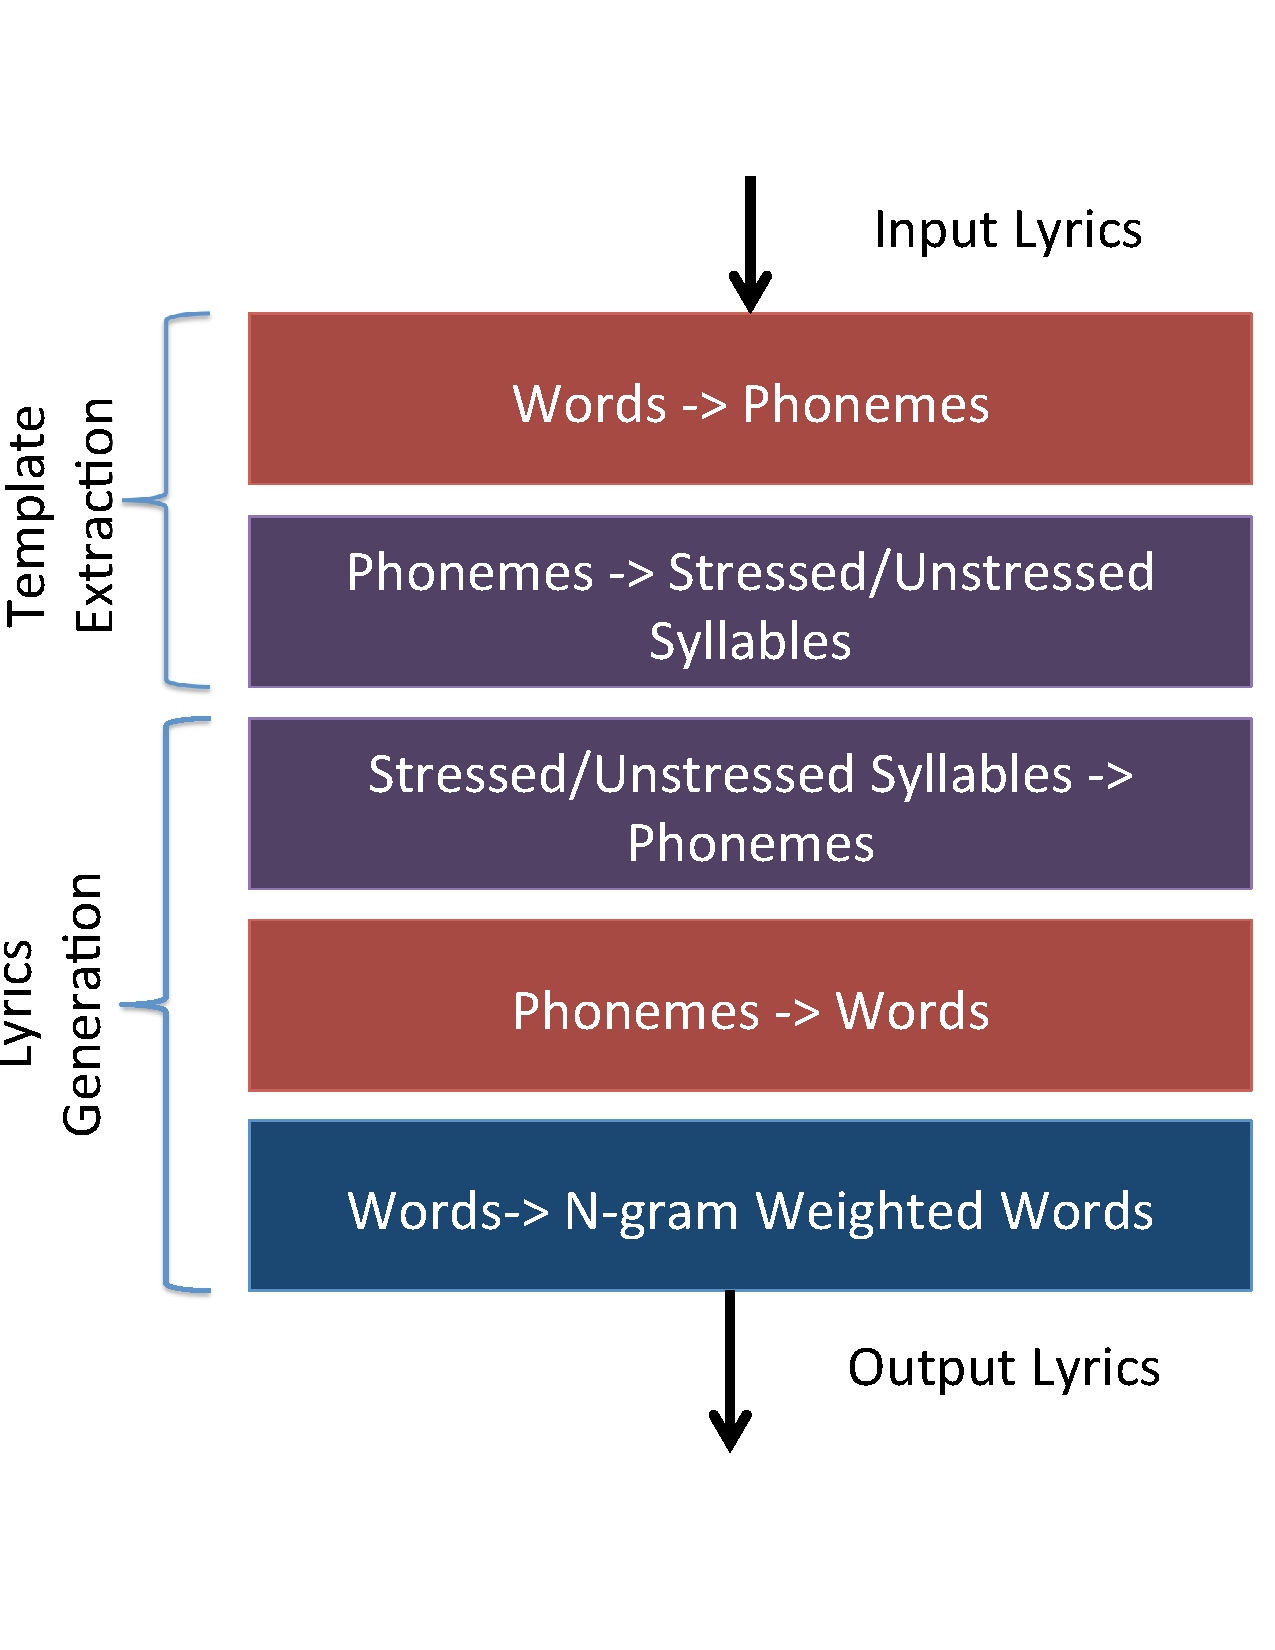
\includegraphics[width=0.3\textwidth]{images/pdf/pipeline.pdf}
\caption{Lyrics Generation Pipeline}
\label{fig:pipeline}
\end{figure}

Our lyrics generation pipeline is as follows. First the user provides
a set of music lyrics in text form as input to our system. The
lyrics are parsed line by line into their representative phonemes,
and then reduced to their basic syllable pattern.
Each syllable pattern is transformed back into all of its possible
phoneme sequences, which are then translated into all possible 
word combinations with the phonemes. These words sequences are weighted with
an n-gram model and ranked to return the most likely
candidate lyrics. The resulting lyrics should have very
similar, if not the same syllable structure as the original
input lyrics.

Our entire pipeline is achieved using only a series of
generated or composed FSTs. Figure~\ref{fig:pipeline}
shows the organization of our pipeline.
The rest of this section is devoted to describing
in detail each aspect of our lyrics generation pipeline.

\subsection{Music Lyrics Data Set and N-Gram Language Model}
The Guardian published a series of articles presenting 1000 songs ``everyone must hear''~\cite{guardian}.
Each article in the series focused on a theme of music, such as love songs or political songs.
They also provided a spreadsheet listing all 1000 of the songs they mentioned in their articles
on their data blog\cite{guardian2}. This
data contained the theme assigned to the song in the articles,
song title, artist name, year the song was released, and a Spotify~\cite{spotify} url.

We used this data to gather song lyrics from the ChartLyrics database~\cite{chartlyrics},
which resulted in a music lyrics corpus containing just over 800 songs. The corpus
contains 12659 unique words, including capitalization, and 10600 words
ignoring capitalization. Some of these are not real words.

We used the n-gram generation tools in the SRI Language Modeling Toolkit to build
an n-gram language model on our music lyrics corpus. We then use the
\texttt{fst\_from\_ngram} tool from
the MIT Finite-State Transducer (FST) Toolkit to produce
an FST from the n-gram model. This approach was also used to build
models on the Brown Corpus for comparison.

\subsection{Syllable Template Extraction}
To extract a syllable template from input lyrics for generating
new lyrics, we need three FSTs: one FST to represent the lyric,
one to map words to phonemes, and
another to map phonemes to stressed/unstressed syllables.
We use the MIT Finite-State Transducer (FST) Toolkit
to transform each line of lyrics into an FST on the fly.

To produce the second FST, we extracted
the Brown Corpus dictionary from the CRYSTAL lexicon
analysis tool used in Assignment 1, which was already
provided in FST form. The closure operation for FSTs
is performed on the word-to-phoneme FST to allow for
generation of arbitrarily many words.

The last necessary FST was produced by hand. The rules for mapping
phonemes to stressed/unstressed syllables
are available in the CRYSTAL source code, and these
rules were used to produce an FST.

Algoritm[x] shows how we put these FSTs together to generate a syllable template.
To generate the template, the input text is split into individual lines, and
each line is transformed into a word-word FST.
This FST is then composed with the word-to-phoneme FST
to retrieve the phoneme structure of the lyric in FST
form. The resulting FST is then composed with the phonemes-to-syllables
FST to produce the final syllable template. This template is then
passed to the lyric generation section of our pipeline to produce
new lyrics.

\subsection{Lyric Generation}
The lyrics generation portion of our pipeline takes as input
a syllable template, and generates as output word sequences
weighted by an n-gram language model. We need the inverse
of both the word-to-phoneme and phonemes-to-syllable
FSTs from template extraction. We used the MIT Finite-State
Transducer (FST) Toolkit to produce these inverse FSTs.
In addition, we need the FST produced using our n-gram language
model built from our music lyrics corpus.

The syllable template
is split into lines, one line for each line in the original
lyrics. Note that the syllable template is in FST form, as
described in the previous section. This syllable template
FST is composed with the inverse of the phonemes-to-syllables
FST to produce all possible phoneme sequences associated
with the syllable template. The resulting FST is then
composed with the inverse of the phonemes-to-words FST
to generate all possible word sequences for the given
phoneme sequences.

At this point, the FST currently contains
old weights from the template extraction phase from when
the original lyrics were mapped to phonemes. These weights
must be removed to properly weight the FST by the n-gram
weights for our music lyrics model. The cleaned word sequence FST
is then composed with the n-gram FST to re-weight
the FST according to the frequencies in our lyrics n-gram model.
The last step can be performed on any FST generated from an n-gram
model, for example a model generated using the Brown Corpus.

\begin{figure}%[htbp]
\centering
%\epsfig{file=images_fixed/eps/architecture.eps,width=0.3\textwidth}
\includegraphics[width=0.3\textwidth]{images/png/lion_king2.png}
\caption{Website Interface for Lyrics Generator.}
\label{fig:interface}
\end{figure}

\begin{figure}%[htbp]
\centering
%\epsfig{file=images_fixed/eps/architecture.eps,width=0.3\textwidth}
\includegraphics[width=0.2\textwidth]{images/png/choose_corpus.png}
\caption{Menu for Choosing a Corpus}
\label{fig:corpus-menu}
\end{figure}

\begin{figure}%[htbp]
\centering
%\epsfig{file=images_fixed/eps/architecture.eps,width=0.3\textwidth}
\includegraphics[width=0.15\textwidth]{images/png/choose_lyrics_menu.png}
\caption{Menu for Choosing New Lyrics}
\label{fig:lyrics-menu}
\end{figure}


\section{Results}
\label{sec:results}
\begin{figure}[t]
\centering
%\epsfig{file=images_fixed/eps/architecture.eps,width=0.3\textwidth}
\includegraphics[width=0.3\textwidth]{images/png/yellow_submarine4.png}
\caption{Results from producing lyrics from the music lyrics data set for ``Yellow Submarine'' by the Beatles}
\label{fig:beatles}
\end{figure}


\subsection{Experimental Setup}
To test our lyrics generation techniques, we built a light-weight
web application using the methods described in Section~\section{sec:methods}.
Figure~\ref{fig:interface} shows the layout of our web interface.
To use the lyrics generator interface, the user pastes lyrics tirectly
into the textbox near the top of the screen, and chooses a corpus
from the menu above the text box shown in Figure~\ref{fig:interface}. To generate new lyrics, the user
presses the ``Make new words!'' button. The text and chosen
corpus are submitted to our back-end server for execution. When
new lyrics are ready, they are presented on the screen as a
list of drop-down menus alongside each line of the original song.
The user can choose a line of lyrics from each drop-down menu to replace
the corresponding line from the original lyrics.
The final set of parody lyrics are printed at the very bottom of the screen
alongside the original lyrics for comparison.

We built FSTs over several n-gram language models to test our lyrics generator:
\begin{itemize}
  \item the entire lyrics data set
  \item the entire Brown Corpus
  \item the science fiction text of the Brown Corpus
  \item the mystery text of the Brown Corpus
  \item the romance text of the Brown Corpus
\end{itemize}

\noindent{
Our lyrics generation pipeline is executed on-the-fly using a series
of piped operations from the Finite-State Transducer (FST) Toolkit on
the back-end server. Our experiments were run locally on our personal
computers.
}

\subsection{Generating Lyrics}
We did not have a clear, quantitative metric for gauging good lyrics
generation. Similarly, it is very noticeable, though perhaps not directly
measureable, when our lyrics generator is producing non-standard
English results. Thus we highlight in this section specific examples
of using the ``Wired Al Yankovic'' parody
lyrics genrator, and discuss the associated successes and
challenges generating music lyrics for our music lyrics corpus
and the Brown Corpus.

\subsection{Music Lyrics Data Set}
Figures~\ref{beatles}, \ref{nsync} and \ref{britney}
are examples of using ``Wired Al'' to generate lyrics for
three well-known songs. The first is
``Yellow Submarine'' by the Beatles. As you can see in
Figure~\ref{beatles}, our lyrics generator successfully
matches the syllable structure of the original input lyrics,
and shows a reasonable blend of multiple songs. However,
issues commonly encountered when using n-gram models,
such as word sequences that do not actually produce
valid sentences or lyrics, are still a problem
for our lyrics generator. This is evident in the
first line, which starts with the word ``and'',
and produces a repetitive, run-on lyric. Note also that for
all three examples, some words needed to be replaced with
syllable markers, as our generator did not recognize
some of the vocabulary used.

Though not completely successful generating lyrics for
``Yellow Submarine'', ``Wired Al'' successfully generates
reasonable lyrics for the `N Sync song ``Tearin' Up My
Heart'', and ``Baby One More Time'' by Britney Spears.
The generated lyrics are not as sophisticated as the
original lyrics, but they make entertaining songs
that can be sung to the tune of the original lyrics,
meeting our goals for good parody lyrics generation.

\begin{figure}[t]
\centering
%\epsfig{file=images_fixed/eps/architecture.eps,width=0.3\textwidth}
\includegraphics[width=0.3\textwidth]{images/png/tumh3.png}
\caption{Results from producing lyrics from the music lyrics data set for ``Tearin' Up My Heart'' by
N' Sync}
\label{fig:nsync}
\end{figure}

\begin{figure}[t]
\centering
%\epsfig{file=images_fixed/eps/architecture.eps,width=0.3\textwidth}
\includegraphics[width=0.3\textwidth]{images/png/hmbomt4.png}
\caption{Results from producing lyrics from the music lyrics Corpus for ``Baby One More Time'' by
Britney Spears}
\label{fig:britney}
\end{figure}


\subsection{Brown Corpus}

\begin{figure}[t]
\centering
%\epsfig{file=images_fixed/eps/architecture.eps,width=0.3\textwidth}
\includegraphics[width=0.3\textwidth]{images/png/hotel_california5.png}
\caption{Results from producing lyrics from the Brown Sci-Fi Corpus for ``Hotel California'' by the
Eagles}
\label{fig:eagles}
\end{figure}

\begin{figure}[t]
\centering
%\epsfig{file=images_fixed/eps/architecture.eps,width=0.3\textwidth}
\includegraphics[width=0.3\textwidth]{images/png/hmbomt3.png}
\caption{Results from producing lyrics from the Brown Sci-Fi Corpus for ``Baby One More Time'' by
Britney Spears}
\label{fig:britney2}
\end{figure}

Figures~\ref{fig:eagles} and \ref{fig:britney2} are examples of using our lyrics generator
with the Brown Corpus science fiction text. Interestingly but not surprisingly,
the lyrics generated by the Brown Corpus read more like sentences than actual
song lyrics. The words and phrases unique to the science fiction data set
made for very interesting lyrics. For example, the use of ``atomic bomb''
in generating lyrics for ``Hotel California'' in Figure~\ref{fig:eagles},
and the use of ``hiding'' and ``never slept'' in ``Baby One More Time''
in Figure~\ref{fig:britney2}.

You can see when comparing directly the two sets of generated
lyrics for ``Baby One More Time'' the difference in tone and prose. The Music
lyrics data set produces light-hearted songs that actively include the listener and engage the
listener, but are also more shallow and don't make sense at times.
The Brown Corpus lyrics sound as if the singer is telling a sinister story
about characters unrelated to the singer or listener.

\subsection{Performance}
Our final lyrics generation pipeline consists of 8 stages:
\begin{itemize}
  \item 1: fst from\_string - i gonna be a mighty king
  \item 2: fst compose -t - pocket\_bcf-inverted-closure.fst -
  \item 3: fst compose -t - phoneme\_to\_stress.fst -
  \item 4: fst compose -t - stress\_to\_phoneme.fst -
  \item 5 fst compose -t - pocket\_bcf-closure.fst -
  \item 6 fst clear\_weights - -
  \item 7 fst compose -t - lyrics-ngram.fst -
  \item 8 fst nbest -s -o -n 30 - -
\end{itemize}

The runtime performance of the ``Wired Al'' lyrics generator for an indidual
line of lyrics is presented
in Figures~\ref{fig:perf1} and \ref{fig:perf2}. We observed that the
total runtime for executing all stages of the lyrics generation
pipeline increased when the number of syllables increases. This is
expected, as an increase in the number of syllables increases
the possible phoneme and word combinations that match the
syllable template.
We see in Figure~\ref{fig:perf2} that
the template extraction half of the pipeline is considerably
cheaper than the lyrics generation half of the pipeline
in terms of runtime. Specifically, stages 5 and 7 take the most
time to perform, which correspond
to mapping phonemes back to words and reweighting the resulting
word sequences using the n-gram language model, respectively.
As the number of syllables increases, it becomes increasingly
more expensive to reweight the final word sequences.

This is also reflected in Figure~\ref{fig:perf3}, which
describes the approximate number of transitions in the
output FST's for each state of the pipeline.
Notice that the number of transitions in stages 5 and 7
is very high, which translates to long execution
times.

\begin{figure}[t]
\centering
%\epsfig{file=images_fixed/eps/architecture.eps,width=0.3\textwidth}
\includegraphics[width=0.3\textwidth]{images/pdf/runtime_by_syllables.pdf}
\caption{Total execution time given number of syllables in a single lyric.}
\label{fig:perf1}
\end{figure}

\begin{figure}[t]
\centering
%\epsfig{file=images_fixed/eps/architecture.eps,width=0.3\textwidth}
\includegraphics[width=0.3\textwidth]{images/pdf/runtime_per_stage.pdf}
\caption{Execution time per stage for lyrics of length 5, 8, 10, 13 and 15 syllables.}
\label{fig:perf2}
\end{figure}
%\section{Improving Lyrics Generation with Latent Semantic Analysis}

\begin{figure}[t]
\centering
%\epsfig{file=images_fixed/eps/architecture.eps,width=0.3\textwidth}
\includegraphics[width=0.3\textwidth]{images/pdf/transitions_per_stage.pdf}
\caption{Approximate number of state transitions per stage for lyrics of length 5, 8, 10, 13 and 15 syllables.}
\label{fig:perf3}
\end{figure}


\section{Conclusions and Future Work}

We presented the design and implementation of ``Wired Al Yankovic'',
an n-gram-based automatic parody lyrics generator. ``Wired Al''
uses a series of FST compositions to transform existing
song lyrics into syllable patterns, and uses these patterns
to generate new lyrics weighted by a given n-gram language model.
We provided anectodal evidence in favor of the of ``Wired Al''
system's ability to generate new song lyrics as well as results
for testing the runtime performance of ``Wired Al'' for
various lengths of word sequences.
%We also present an approach
%to extending our system to include keyword search on the underlying
%corpus using Latent Semantic Analysis.

We hope to grow and refine our music lyrics corpus and add additional
data sets (such as a movie scripts corpus). In addition, we want
to extend the system such that multiple users can interact with
``Wired Al'' simultaneously, and we want to finish a full deployment
of our website, so others can enjoy and learn from our lyrics generation
system.

%% if specified like this the section will be ommitted in review mode
%\acknowledgements{Blank}
%
\bibliographystyle{abbrv}
%%use following if all content of bibtex file should be shown
%\nocite{*}
\bibliography{writeup}
\end{document}
